\documentclass[twoside]{article}
\input{ISC18-english.sty}
\begin{document}
\thispagestyle{empty}
\fancyhead[LE]{The Ising spin model on the square  grid system based on Boltzmann  distribution}
\fancyhead[RO]{M. Shams and M. A. Mirzaie}
\begin{center}
{
\includegraphics [height=25mm, width=150.3mm] {Images/isc18E}} \\
\vspace*{-1.8cm}
\vspace*{4cm}
{\Large \bf The Ising spin model on the square  grid system based on Boltzmann  distribution}\\
{\bf
Mehdi Shams$^1$, Mohammad Ali Mirzaie\footnote[2]{{\bf Corresponding Author:} {\tt m.a.mirzaie@ut.ac.ir}} \\
$^1$Department of Statistics, Faculty of Mathematical Sciences, University of Kashan, Kashan, Iran\\
$^2$School of Mathematics, Statistics, and Computer Science, College of Science, University of Tehran, Tehran, Iran}
\end{center}
\rule{\textwidth}{0.2mm}\\
\noindent{\bf Abstract:}\\ 
Many scientific disciplines have adopted the Ising model as a fundamental physical framework. Three specific configurations of this model are examined in this paper, with emphasis on the square $n \times n$ grid. For general Ising models built upon the Boltzmann stationary distribution, we show that the maximum likelihood estimator coincides with the method-of-moments estimator for the inverse temperature parameter $\beta$. Analytical solution of the resulting equation proves impossible; hence linear regression methods are employed to obtain these estimates. A general condition governing convexity of the Boltzmann probability entropy is also put forward.

\noindent{\bf Keywords:} Entropy, Boltzmann distribution, maximum likelihood estimator, regression models, induced probability vector. \\
\noindent{\bf Mathematics Subject Classification (2010):} $\rm 62B10$, $62F10$, $62P35$, $62M10$. \\
\hspace{1cm}\rule{\textwidth}{0.2mm}\\

\section{Introduction}
Ferromagnetism finds a mathematical representation in the Ising model within statistical mechanics. This model extends beyond physics into machine learning, image processing, and economics. Ernst Ising first proved that no phase transition toward a ferromagnetic ordered state occurs in one dimension at any finite temperature. A comprehensive review of Ising models in ferromagnetic and other physical contexts appears in \cite{30}. Two possible orientations exist for each spin: upward or downward, corresponding respectively to alignment with or opposition to the external field. A quantum feedback variant of the Ising model received investigation in \cite{24}. Phase separation, wetting and dewetting phenomena, lattice-based liquid-gas systems, and spin glasses represent some areas where this model has been applied. Industrial applications also utilize elementary Ising spin models to represent cascading failures within networks \citep{21}.  

The Ising model on a square $n \times n$ grid constitutes a particularly noteworthy special case, which we analyze in Section \ref{sec3}. There we prove the equivalence of the maximum likelihood and method-of-moments estimators for $\beta$, compute these estimates via linear regression, derive the system entropy, state the convexity condition for the Boltzmann entropy, obtain the probability vectors induced by the system energies, and show that both entropies are even functions of $\beta$. Section \ref{sec6} then discusses the results, offers recommendations, and outlines directions for future research.

\section{The Ising model on the grid system} \label{sec3}
This section defines the Ising model on a grid and derives its main probabilistic properties.

One important stationary distribution in physics has the form
\begin{equation} \label{3.3}
{{\xi }_{x}}=\frac{{{e}^{-\beta {{E}_{x}}}}}{\sum\nolimits_{y\in E}{{{e}^{-\beta {{E}_{y}}}}}}
\end{equation}
where ${{E}_{x}}$ denotes the energy of state $x$, while the normalization constant $\beta$ represents the inverse temperature characteristic of the heat baths. State occupation in physical particles (atoms or molecules) and biological systems is described by the Boltzmann distribution. State $x$ with energy ${{E}_{x}}$ receives probability proportional to ${{e}^{-\beta {{E}_{x}}}}$, where $\beta =\tfrac{1}{{{k}_{B}}T}$, $T$ stands for temperature in Kelvin, and ${{k}_{B}}$ denotes the Boltzmann constant \citep{6}.

Magnetism modeling and image processing in physical research have utilized the Ising model. A graph $G$ consisting of edges is considered, with each site $i$ assigned a spin of $+1$ or $-1$. Hence ${{x}_{i}}=\pm 1$ holds for every $i$. A square $n\times n$ grid is now considered, where each point connects to four neighbors. Consequently $k={{2}^{{{n}^{2}}}}$ possible states exist, so $E=\{ E_{x_1},...,E_{x_k}\}$. Energy definition for each state $x \in \{ x_1,...,x_k\}$ is $E_x=-\sum\nolimits_{i\sim j} x_i x_j$, with summation running over all neighboring site pairs $i$ and $j$. The $3\times 3$ grid Ising model contains ${{2}^{9}}=512$ states, and energy computation for each of these 512 states is feasible. For instance, the configuration $x= \left(-1, -1, 1, 1, 1, -1, -1, 1, 1\right)$ possesses energy
$E_x = -\sum\nolimits_{i\sim j} x_i x_j = -\sum\nolimits_{(m,n)\sim (v,w)} a_{mn} a_{vw} = 4$.
All energies in the $3\times 3$ grid Ising model average to zero; that is, $\tfrac{1}{512}\sum\nolimits_{i=1}^{512}{{{E}_{{{x}_{i}}}}}=0.$

We now inquire about the expected value of the energy random variable under the probability function specified in \eqref{3.3}. Computation yields
$e(\beta) = {{\boldsymbol{E}}_{\beta }}\left( {{E}_{x}} \right)=\frac{\sum\nolimits_{x\in E}{E_{x}^{{}}{{e}^{-\beta {{E}_{x}}}}}}{\sum\nolimits_{y\in E}{{{e}^{-\beta {{E}_{y}}}}}}$.
Energy variance follows as
\[v(\beta)={\boldsymbol{Var}}_\beta(E_x) = \boldsymbol{E}_\beta(E_x^2) - \Big(\boldsymbol{E}_\beta(E_x)\Big)^2 = \sum\nolimits_{x \in E} E_x^2 \frac{e^{-\beta E_x}}{\sum\nolimits_{y \in E} e^{-\beta E_y}} - \left(\frac{\sum\nolimits_{x \in E} E_x e^{-\beta E_x}}{\sum\nolimits_{y \in E} e^{-\beta E_y}}\right)^2.\]
Within the $3 \times 3$ grid model, ${\boldsymbol{E}_{\beta }}\left( {{E}_{x}} \right)$ exhibits decreasing behavior with respect to $\beta$. Furthermore, ${\boldsymbol{E}_{\beta }}\left( E_{x}^{2} \right)$ decreases when $\beta <0$ and increases when $\beta >0$. Dispersion ${\boldsymbol{Var}_{\beta }}\left( {{E}_{x}} \right)$ reaches higher levels for $\beta$ near zero (approximately $\beta \in \left[-2,2\right]$) and lower levels for $\beta$ distant from zero on either side (approximately $\left| \beta \right|>2$). Symmetry about zero characterizes the energy distribution in the $3\times 3$ grid model (for all $\beta$), giving
\begin{equation} \label{5.1}
e(-\beta) = \boldsymbol{E}_{-\beta}(E_x) = \frac{\sum\nolimits_{x \in E} E_x e^{\beta E_x}}{\sum\nolimits_{y \in E} e^{\beta E_y}} = -\frac{\sum\nolimits_{x \in E} E_x e^{-\beta (-E_x)}}{\sum\nolimits_{y \in E} e^{-\beta E_y}} = -\frac{\sum\nolimits_{x \in E} E_x e^{-\beta E_x}}{\sum\nolimits_{y \in E} e^{-\beta E_y}} = -e(\beta)
\end{equation}
and also ${{e}_{2}}(-\beta) = {\boldsymbol{E}_{-\beta}}\left( E_{x}^{2} \right) = \frac{\sum\nolimits_{x\in E} E_{x}^{2} e^{-\beta E_{x}}}{\sum\nolimits_{y\in E} e^{-\beta E_{y}}} = {{e}_{2}}(\beta)$, and 
\[v(-\beta) = \boldsymbol{Var}_{-\beta}\left( E_{x} \right) = {{e}_{2}}(-\beta) - \left( e(-\beta) \right)^{2} = {{e}_{2}}(\beta) - \left( e(\beta) \right)^{2} = v(\beta).\] Hence, within the $3\times 3$ grid model, $e(\beta )={\boldsymbol{E}_{\beta }}\left( {{E}_{x}} \right)$ proves odd, while ${{e}_{2}}(\beta )={\boldsymbol{E}_{\beta }}\left( E_{x}^{2} \right)$ and $v(\beta )={\boldsymbol{Var}_{\beta }}\left( {{E}_{x}} \right)$ prove even.

A probability mass function on $E$ is defined by the Boltzmann distribution through \eqref{3.3}. When $\beta =0$, the distribution in \eqref{3.3} simplifies to the discrete uniform distribution $DU\left\{ 1,...,512 \right\}$, i.e., ${{\xi }_{x}}=\tfrac{1}{512}$ for ${{E}_{x}}={{E}_{{{x}_{1}}}},...,{{E}_{{{x}_{512}}}}$.

For any arbitrary state $x$, each site $i$ follows a uniform distribution. Updating of the spin at that site proceeds from the conditional distribution of that site given the remaining sites of $x$. Denote the sites by $1,\ldots,m$ and the spin at site $k$ by $x_k$, while ${\boldsymbol{x}}_{-k}=\left( x_1,...,x_{k-1},x_{k+1},...,x_m \right)$ represents the other $m-1$ sites. For fixed $k$, define ${\boldsymbol{x}}^+=\left( x_1,...,x_{k-1},+1, x_{k+1},...,x_m \right)$ and ${\boldsymbol{x}}^-=\left(x_1,...,x_{k-1},-1,x_{k+1},...,x_m \right)$. Then:
\begin{small}
\begin{align*}
d_k(\beta) &= P\left( x_k = +1 \,\middle|\, \boldsymbol{x}_{-k} \right) \\
&= \frac{\xi_{x^+}}{\xi_{x_{-k}}} = \frac{\xi_{x^+}}{\xi_{x^+} + \xi_{x^-}} \\
&=\frac{1}{1 + e^{\beta \left( E_{x^+} - E_{x^-} \right)}} = \frac{1}{1 + e^{-2\beta \sum\nolimits_{i \sim k} x_i}} \\
&= {\sigma }_{0 ,\beta} (2\sum\nolimits_{i \sim k} x_i) \\
&= \begin{cases}
    \frac{1}{2} & k = 1, 5, 9 \\
   {\sigma }_{0 ,\beta}(2) & k = 2, 8 \\
     {\sigma }_{0 ,\beta}(-2) & k = 4 \\
      {\sigma }_{0 ,\beta}(6) & k = 6 \\
     {\sigma }_{0 ,\beta}(-4) & k = 3 \\
     {\sigma }_{0 ,\beta}(4) & k = 7
\end{cases}
\end{align*}
\end{small}
where ${{E}_{{{\boldsymbol{x}}^{+}}}}=-\Big( \sum\nolimits_{\begin{smallmatrix} i\sim j \\ i,j\ne k \end{smallmatrix}}^{{}}{{{x}_{i}}{{x}_{j}}}+\sum\nolimits_{\,\,\,i\sim k}{{{x}_{i}}} \Big)$, ${{E}_{{{\boldsymbol{x}}^{-}}}}=-\Big( \sum\nolimits_{\begin{smallmatrix} i\sim j \\ i,j\ne k \end{smallmatrix}}^{{}}{{{x}_{i}}{{x}_{j}}}-\sum\nolimits_{\,\,\,i\sim k}{{{x}_{i}}} \Big)$, and ${\sigma }_{a ,b }( x )=\frac{1}{1+{{e}^{-b ( x-a )}}}$ defines a sigmoid function with parameters $a$ and $b$. Also,
\[d'_k(\beta) = P\left( \boldsymbol{x}_k = -1 \,\middle|\, \boldsymbol{x}_{-k} \right) = 1 - P\left(\boldsymbol{x}_k = +1 \,\middle|\, \boldsymbol{x}_{-k} \right) = \frac{1}{1 + e^{2\beta \sum\nolimits_{i \sim k} x_i}}.\]

Because $d_k(-\beta) = 1 - d_k(\beta)$, the curve ${{d}_{k}}\left( \beta \right)$ displays central symmetry around the point $(0,0.5)$. Conditional mathematical expectation follows from
%\begin{small}
%\[
%e_k\left( \beta \right) = {{\boldsymbol{E}}_{\beta }}\left( {{x}_{k}} \,\middle|\, {{\boldsymbol{x}}_{-k}} \right) = \sum\nolimits_{i\in \{-1,1\}} i \times P\left( {{x}_{k}}=i \,\middle|\, {{\boldsymbol{x}}_{-k}} \right) = \frac{1 - e^{-2\beta \sum\nolimits_{i\sim k}{{{x}_{i}}}}}{1 + e^{-2\beta \sum\nolimits_{i\sim k}{{{x}_{i}}}}} = \begin{cases}
%    0 & k = 1, 5, 9 \\
%    \frac{1 - e^{-2\beta}}{1 + e^{-2\beta}} & k = 2, 8 \\
%    \frac{1 - e^{2\beta}}{1 + e^{2\beta}} & k = 4 \\
%    \frac{1 - e^{-6\beta}}{1 + e^{-6\beta}} & k = 6 \\
%    \frac{1 - e^{4\beta}}{1 + e^{4\beta}} & k = 3 \\
%    \frac{1 - e^{-4\beta}}{1 + e^{-4\beta}} & k = 7
%\end{cases}
%\]
%\end{small}
\begin{align*}
e_k\left( \beta \right) &= {{\boldsymbol{E}}_{\beta }}\left( {{x}_{k}} \,\middle|\, {{\boldsymbol{x}}_{-k}} \right)\\
&= \sum\nolimits_{i\in \{-1,1\}} i \times P\left( {{x}_{k}}=i \,\middle|\, {{\boldsymbol{x}}_{-k}} \right) 
&= \frac{1 - e^{-2\beta \sum\nolimits_{i\sim k}{{{x}_{i}}}}}{1 + e^{-2\beta \sum\nolimits_{i\sim k}{{{x}_{i}}}}} \\
&= \begin{cases}
    0 & k = 1, 5, 9 \\
    \frac{1 - e^{-2\beta}}{1 + e^{-2\beta}} & k = 2, 8 \\
    \frac{1 - e^{2\beta}}{1 + e^{2\beta}} & k = 4 \\
    \frac{1 - e^{-6\beta}}{1 + e^{-6\beta}} & k = 6 \\
    \frac{1 - e^{4\beta}}{1 + e^{4\beta}} & k = 3 \\
    \frac{1 - e^{-4\beta}}{1 + e^{-4\beta}} & k = 7
    \end{cases}
\end{align*}

Using the sigmoid function, $e_k\left( \beta \right)$ can be rewritten as $e_2\left( \beta \right)=e_8\left( \beta \right)={\sigma }_{0 ,\beta}(2)-{\sigma }_{0 ,\beta}(-2)=-e_4\left( \beta \right)$, $e_6\left( \beta \right)={\sigma }_{0 ,\beta}(6)-{\sigma }_{0 ,\beta}(-6)$, and $e_7\left( \beta \right)={\sigma }_{0 ,\beta}(7)-{\sigma }_{0 ,\beta}(-7) =-e_3\left( \beta \right)$. Observation yields \[e_k(-\beta) = 2d_k(-\beta) - 1 = 1 - 2d_k(\beta) = -e_k(\beta)\] indicating oddness of ${{e}_{k}}\left( \beta \right)$; equivalently, central symmetry about the origin holds.

We now compute the conditional variance using an analogous approach. Since
\[{{\boldsymbol{E}}_{\beta }}\left( x_{k}^{2}|{{x}_{-k}} \right)=\sum\nolimits_{i\in \left\{ -1,1 \right\}}{{{i}^{2}}\times P\left( {{x}_{k}}=i|{{\boldsymbol{x}}_{-k}} \right)}={{d}_{k}}\left( \beta \right)+{{{d}'}_{k}}\left( \beta \right)={{d}_{k}}\left( \beta \right)+\left( 1-{{d}_{k}}\left( \beta \right) \right)=1,\]
we obtain
\[
v_k(\beta) = {\boldsymbol{Var}_{\beta }}\left( {{x}_{k}}|{\boldsymbol{x}_{-k}} \right) =
\begin{cases}
    1 & k = 1, 5, 9, \\
    \frac{4e^{-2\beta}}{(1 + e^{-2\beta})^2}=4{\sigma }_{0 ,\beta}(2)\big(1-{\sigma }_{0 ,\beta}(2)\big) & k = 2, 4, 8 \\
    \frac{4e^{4\beta}}{(1 + e^{4\beta})^2}=4{\sigma }_{0 ,\beta}(-4)\big(1-{\sigma }_{0 ,\beta}(-4)\big) & k = 3, 7 \\
    \frac{4e^{-6\beta}}{(1 + e^{-6\beta})^2}=4{\sigma }_{0 ,\beta}(6)\big(1-{\sigma }_{0 ,\beta}(6)\big) & k = 6
\end{cases}
\]
One can readily verify that \[{{v}_{k}}\left( -\beta \right)=1-{{\left( {\boldsymbol{E}_{-\beta }}\left( {{x}_{k}}|{\boldsymbol{x}_{-k}} \right) \right)}^{2}}=1-{{\left( -{{e}_{k}}\left( \beta \right) \right)}^{2}}={{v}_{k}}\left( \beta \right).\] Hence ${{v}_{k}}\left( \beta \right)$ is an even function, exhibiting axial symmetry about the vertical axis.

When $\beta =0$, the three functions ${{d}_{k}}\left( \beta \right)$, ${{e}_{k}}\left( \beta \right)$, and ${{v}_{k}}\left( \beta \right)$ no longer depend on $\beta$; this occurs precisely for the diagonal positions of the $3\times 3$ grid matrix, i.e., points 1, 5, and 9.
 Thus ${{d}_{1}}\left( 0 \right)={{d}_{5}}\left( 0 \right)={{d}_{9}}\left( 0 \right)=\tfrac{1}{2}$, ${{e}_{1}}\left( 0 \right)={{e}_{5}}\left( 0 \right)={{e}_{9}}\left( 0 \right)=0$, and ${{v}_{1}}\left( 0 \right)={{v}_{5}}\left( 0 \right)={{v}_{9}}\left( 0 \right)=1$.

We now compute the entropy of the distribution given in \eqref{3.3}. Entropy definition gives
\[H_{\beta}(\boldsymbol{\xi}) = -\sum\nolimits_{x \in E} \xi_x \ln \xi_x = \beta \boldsymbol{E}_{\beta}(E_x) + \ln \left( \sum\nolimits_{y \in E} e^{-\beta E_y} \right).\]

\begin{pro} \label{pro3.7}
\citep{shams}. Under the constraints $\sum\nolimits_{i=1}^{n}{{{\xi }_{i}}}=1$ and $\boldsymbol{E}\left( {{E}_{x}} \right)=\sum\nolimits_{i=1}^{n}{{{\xi }_{i}}}{{E}_{i}}=c$, the unique maximizer of entropy $H(\boldsymbol{\xi })=-\sum\nolimits_{i=1}^{n}{{{\xi }_{i}}}\ln {{\xi }_{i}}$ is the Boltzmann distribution.
\end{pro}

For which $\beta$ values does the entropy function ${{H}_{\beta }}(\boldsymbol{\xi })$ become convex or concave? The following proposition provides the answer.

\begin{pro} \label{pro3.5}
\citep{shams}. For the Ising model, the entropy of the Boltzmann distribution defined in \eqref{3.3} is convex with respect to $\beta$ whenever the condition
\begin{small}
$\beta \mathbf{Cov}{\beta} \left( E_x, E_x^2 \right) \geq \mathbf{Var}{\beta} \left( E_x \right) \left( 2\beta \boldsymbol{E}_{\beta} \left( E_x \right) + 1 \right)$
\end{small}
is satisfied.
This inequality can be rewritten using the third central moment as
\begin{small}
$\beta {\boldsymbol{E}_{\beta}}{{\Big( {{E}_{x}}-{\boldsymbol{E}_{\beta}}\left( {{E}_{x}} \right) \Big)}^{3}} \ge {{\boldsymbol{Var}}_{\beta}}\left( E_{x}^{{}} \right)$.
\end{small}
\end{pro}

Within the $3\times 3$ grid model, ${{H}_{\beta }}(\boldsymbol{\xi })$ declines as $\left| \beta \right|$ grows. Maximum entropy occurs at $\beta =0$; that is, $\arg {{\max }_{\beta }}{{H}_{\beta }}(\boldsymbol{\xi })=0$, with ${{H}_{0}}(\boldsymbol{\xi })=6.238325$. Symmetry about $\beta =0$ characterizes the entropy function in the $3\times 3$ grid, because by \eqref{5.1} we have
\[h(-\beta) = {{H}_{-\beta }}(\boldsymbol{\xi }) = -\beta e(-\beta) + \ln \left( \sum\nolimits_{y\in E}{{{e}^{-\beta {{E}_{y}}}}} \right) = {{H}_{\beta }}(\boldsymbol{\xi }) = h(\beta).\]
Hence $h(\beta )={{H}_{\beta }}(\boldsymbol{\xi })$ proves even within the $3\times 3$ grid model.

Do MLE and MME for $\beta$ coincide in model \eqref{3.3} based on a random sample? Suppose ${{X}_{1}},\ldots,{{X}_{n}}\overset{i.i.d.}{\mathop{\sim }}\,{{f}_{\theta }}(x)$. Method-of-moments estimation equates sample moments ($\bar{X}=\tfrac{1}{n}\sum\nolimits_{i=1}^{n}{{{X}_{i}}}$) with theoretical moments (${\boldsymbol{E}_{\theta }}\left( X \right)=\sum\nolimits_{x}{x{{f}_{\theta }}(x)}$). The resulting $\tilde{\theta }$ is called the MME for $\theta$. Consider the likelihood function $\boldsymbol{L} \left( \theta \right)=\prod\nolimits_{i=1}^{n}{{{f}_{\theta }}(x)}$. Then $\hat{\theta }$ qualifies as an MLE for $\theta$ when $\hat{\theta} = \arg\max_{\theta} \boldsymbol{L}(\theta)$, i.e., $\boldsymbol{L}(\hat{\theta}) = \max_{\theta} \boldsymbol{L}(\theta)$. Equality of MME and MLE computed from the first moment for $\beta$ is proved in the following theorem.

\begin{thm} \label{theorem3.8}
\citep{shams}. Within the $3\times 3$ grid Ising model, the MLE and MME for $\beta$ are identical.
\end{thm}

Define $r\left( \beta \right) = {\boldsymbol{E}_{\beta }}\left( {{E}_{x}} \right) - {{\bar{E}}_{x}} = \frac{\sum\nolimits_{y\in E}{{{E}_{y}}{{e}^{-\beta {{E}_{y}}}}}}{\sum\nolimits_{y\in E}{{{e}^{-\beta {{E}_{y}}}}}} - {{\bar{E}}_{x}}$.
Theorem \ref{theorem3.8} shows that solving $r\left( \beta \right)=0$ produces both MME and MLE for $\beta$. Numerical methods become necessary because analytical solution of this equation proves impossible. Regression models offer one approach to finding the root of $r\left( \beta \right)=0$ for the $3\times 3$ grid model.

The procedure operates as follows. Random samples drawn from distribution \eqref{3.3} yield averages ${{\bar{E}}_{x}}$. Substituting these values into $r\left( \beta \right)=0$ determines the root. This process generates pairs consisting of average energy and corresponding root value. Treating average energy as independent variable and root value as dependent variable within regression models reveals a linear relationship between these two quantities. Hence the regression model supplies the root of $r\left( \beta \right)=0$, which exactly equals the MME and MLE for $\beta$.

For the $3\times 3$ grid, the regression model takes the form
$\hat{\beta} = \tilde{\beta} = -0.0739403 \bar{E}_x$.
The $R^{2}$ value of 0.9978 for this model indicates very strong linearity.

\begin{table}[h]
\centering
\begin{tabular}{|c|c|c|}
\hline
\textbf{energy} & \textbf{number} & \textbf{probabilities} \\ \hline
-12 (12) & 2 & 0.00390625 \\
-8 (8) & 8 & 0.01562500 \\
-6 (6) & 32 & 0.06250000 \\
-4 (4) & 46 & 0.08984375 \\
-2 (2) & 96 & 0.18750000 \\
0 & 144 & 0.28125000 \\
\hline
\end{tabular}
\caption{Frequency table (and probability values) for different energy states (for $\beta =0$) in the $3\times 3$ grid system.}
\label{table5.1}
\end{table}

Let ${{\boldsymbol{\tau }}_{1}}$ denote the probability vector from Table \ref{table5.1} (corresponding to $\beta =0$). We refer to ${{\boldsymbol{\tau }}_{1}}$ as the probability vector induced by the system energies.
 Table \ref{table5.1} shows 144 states possessing zero energy. More generally, the count of states with energy ${{E}_{x}}=2,4,6,8,12$ equals the count with energy ${{E}_{x}}=-2,-4,-6,-8,-12$, respectively. Thus the energy distribution exhibits symmetry about zero for all $\beta$, while the probability distribution shows such symmetry only at $\beta =0$. At $\beta =0$, the random variable supported on $E={{S}_{{{E}_{x}}}}=\left\{ 0,\pm 2,\pm 4,\pm 6,\pm 8,\pm 12 \right\}$ with probability mass function ${{\boldsymbol{\tau }}_{1}}$ from Table \ref{table5.1} has entropy ${{H}_{0}}({{\boldsymbol{\tau }}_{1}})=-\sum\nolimits_{i\in {{S}_{{{E}_{x}}}}}{{{p}_{i}}}\ln {{p}_{i}}=1.937360313.$

\begin{figure}[h] \centering 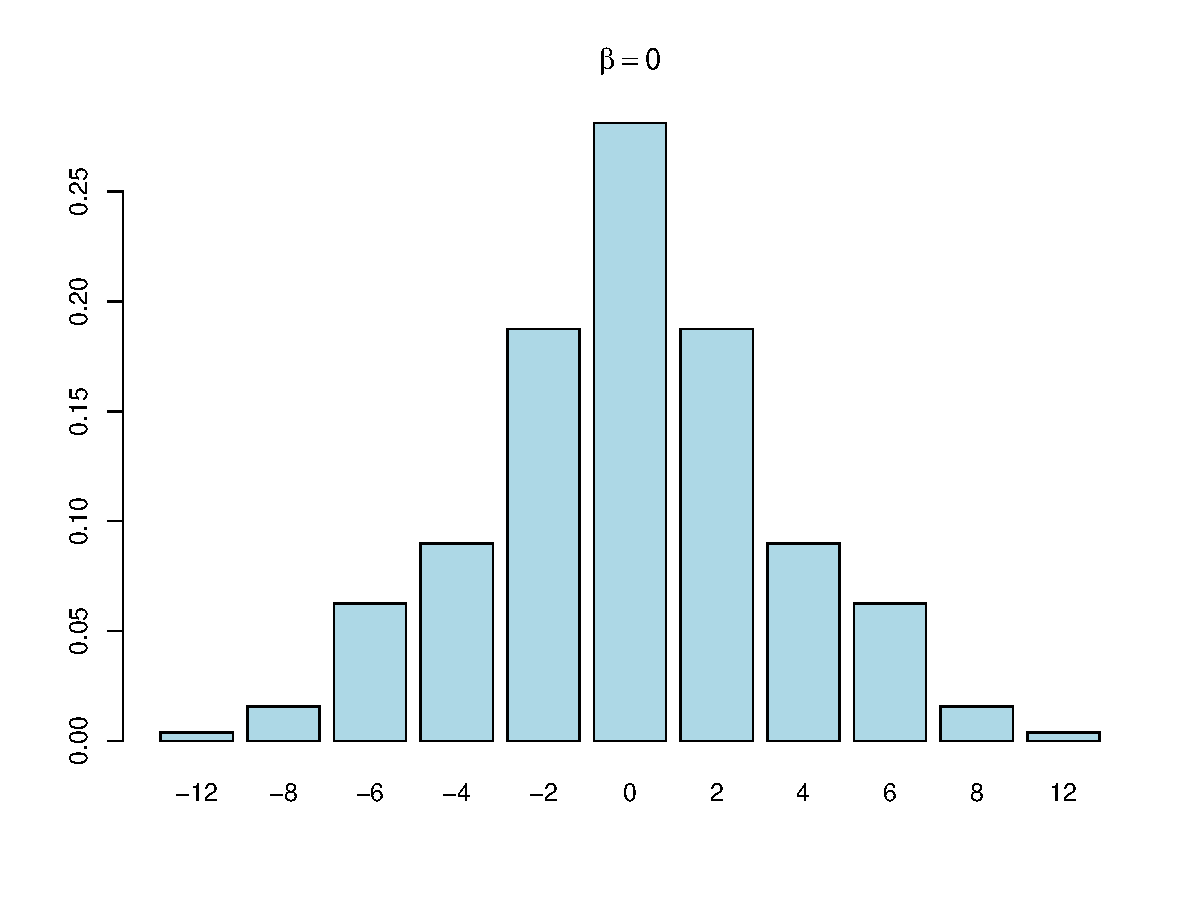
\includegraphics[width=0.49 \textwidth]{fig5.1.pdf} \caption{The probability of obtaining some energies for $\beta =0$ in the $3\times 3$ grid system.} \label{fig24} \end{figure}
\begin{figure}[h] \centering 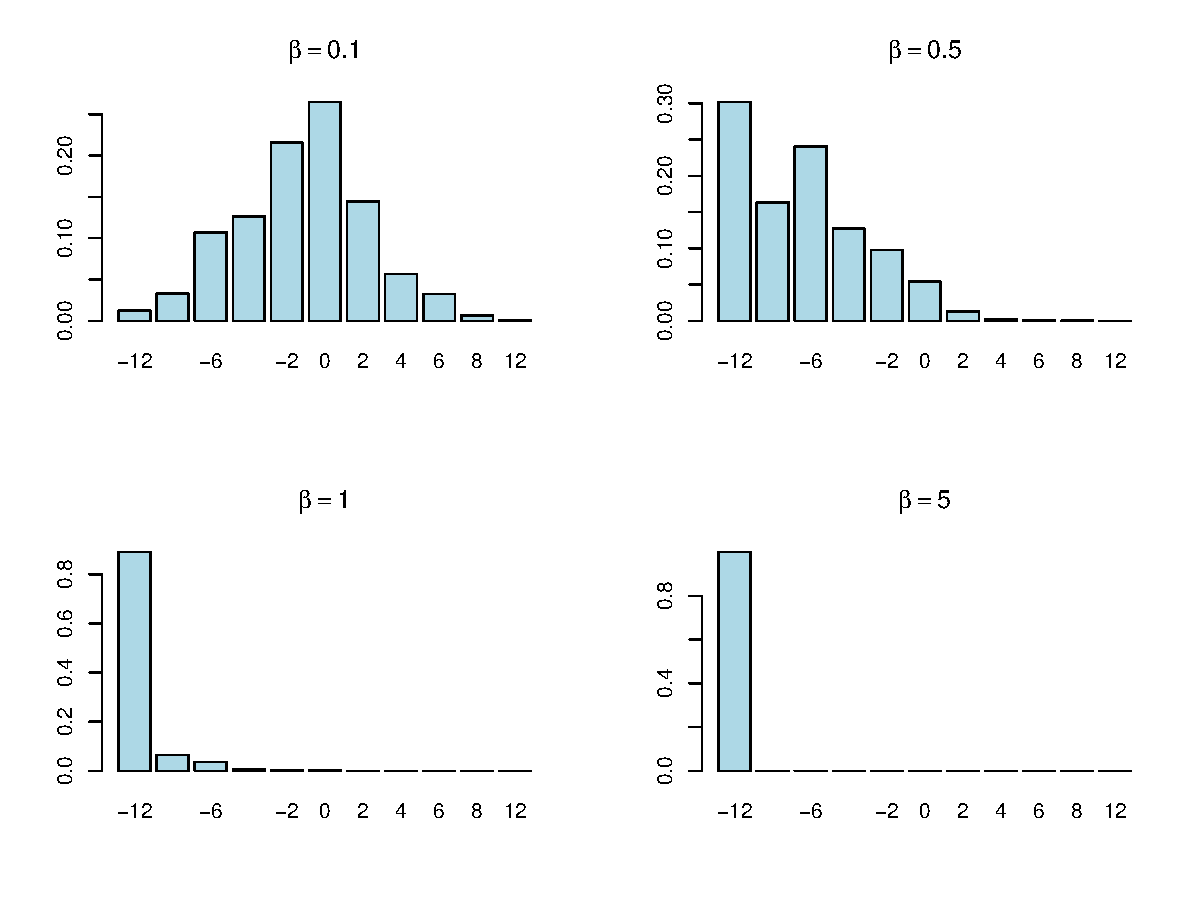
\includegraphics[width=0.49 \textwidth]{fig5.2.pdf} 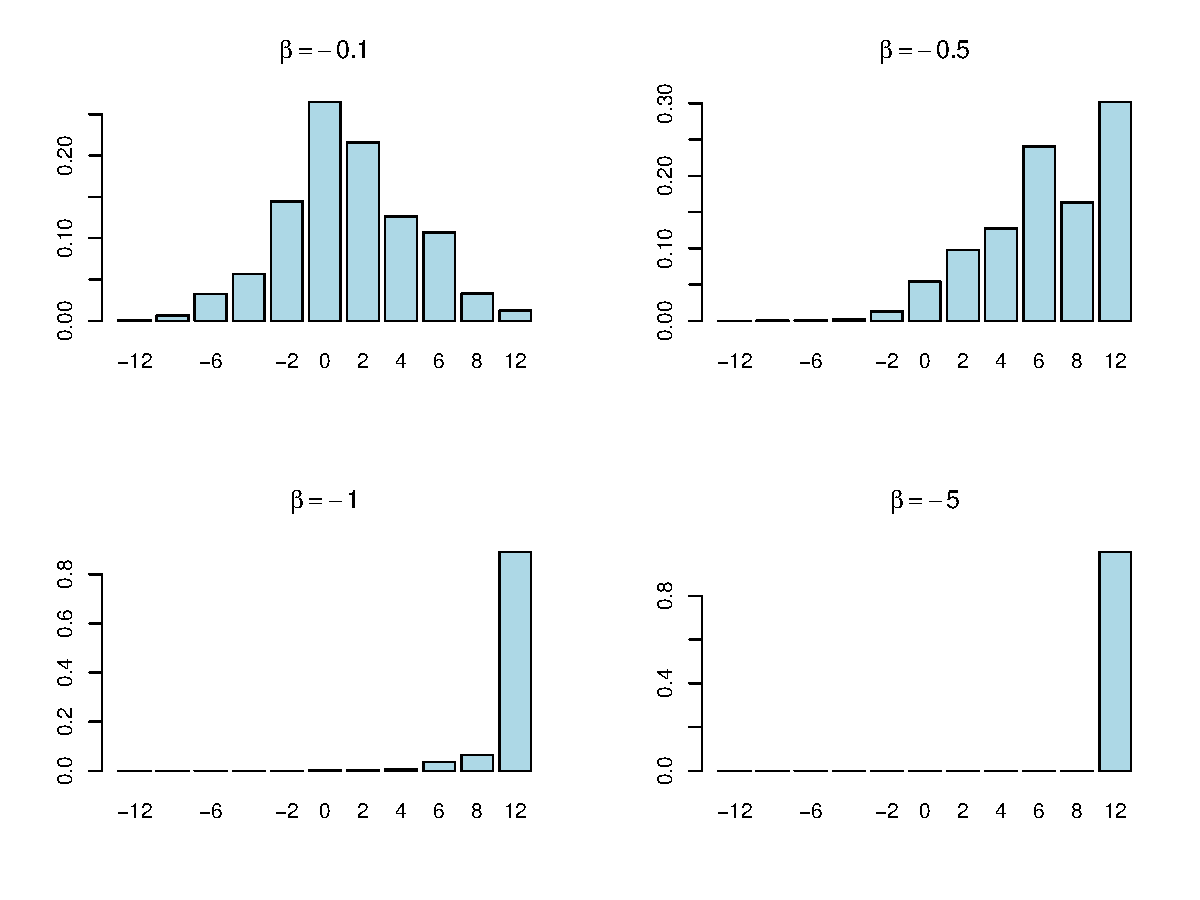
\includegraphics[width=0.5 \textwidth]{fig5.3.pdf} \caption{The probability of obtaining some energies for $\beta >0$ (left) and $\beta <0$ (right) in the $3\times 3$ grid system.} \label{fig25} \end{figure}

Clear observation of probability symmetry appears in Figure \ref{fig24}. Figure \ref{fig25} reveals that for $\beta >0$ (left panel) the distribution ${{\boldsymbol{\tau }}_{1}}$ places greater mass on low-energy states, while for $\beta <0$ (right panel) it places greater mass on high-energy states.

The entropy of the $3\times 3$ grid system is bimodal and symmetric. Specifically, the maximizers occur at $\beta = \pm 0.2252252$, yielding the common value $H_{\pm 0.2252252}(\boldsymbol{\tau}_1) = 1.952689$. Moreover, from Table \ref{table5.1} we obtain
\[h_{{\tau }_{1}}(\beta ) = H_{\beta }({\boldsymbol{\tau }}_{1}) = -\sum\nolimits_{i\in S_{{E}_{x}}} {\boldsymbol{\tau }}_{1}(i) \ln \left( {\boldsymbol{\tau }}_{1}(i) \right) = H_{-\beta }({\boldsymbol{\tau }}_{1}) = h_{{\tau }_{1}}(-\beta )\]
which confirms that ${{h}_{{{\tau }_{1}}}}(\beta )={{H}_{\beta }}({{\boldsymbol{\tau }}_{1}})$ is an even function within the $3\times 3$ grid model.
\section{CONCLUSIONS AND RECOMMENDATIONS} \label{sec6}
 Experimental limitations prevented application of certain statistical inferences in this paper. Overcoming these limitations would enable study of confidence intervals, hypothesis tests, uniformly minimum variance unbiased estimators (UMVUE), minimum risk equivariant estimators (MRE), and other statistical inferences for $\beta$. The equation solved to find MLE for $\beta$ in this paper required statistical methods and regression models for root finding. If experimental limitations were removed and appropriate energy data became available, this problem would be solved and the MLE could be obtained directly.

\begin{thebibliography}{9}
\bibitem[Catanzaro et. al. (2017)]{6}
Catanzaro M.J., Chernyak V.Y. and Klein J.R. (2017), A higher Boltzmann distribution, {\it Journal of Applied and Computational Topology} 1(2), 215-240.
\bibitem[Hooyberghs et. al. (2012)]{21}
Hooyberghs H., Van Lombeek S., Giuraniuc C., Van Schaeybroeck B. and Indekeu J.O. (2012), Ising model for distribution networks, {\it Philosophical Magazine}, 92(1-3), 168-191.
\bibitem[Kiesewetter and Drummond (2022)]{24}
Kiesewetter S. and Drummond P.D. (2022), Coherent Ising machine with quantum feedback: The total and conditional master equation methods, {\it Physical Review A}, 106(2), 022409.
\bibitem[Niss (2005)]{30}
Niss M. (2005), History of the Lenz-Ising model 1920-1950: from ferromagnetic to cooperative phenomena, {\it Archive for History of Exact Sciences}, 59(3), 267-318.
\bibitem[Shams and Mirzaie(2026)]{shams}
Shams M. and Mirzaie M.A. (2026), The Kolmogorov forward equations, information theory and mathematical modeling of the Ising model, {\it Computational Methods for Differential Equations}, 14(1), 421-469.
\end{thebibliography}
\end{document}